\section{Thực nghiệm với mô hình ngôn ngữ và RAG}
\label{subsec:experiment_llm_rag}

\subsection{Thực nghiệm với mô hình ngôn ngữ}
Mục tiêu của thực nghiệm này là đánh giá khả năng của các mô hình ngôn ngữ lớn (LLM) trong việc trả lời câu hỏi trắc nghiệm Lịch sử lớp 12, từ đó xác định giới hạn của phương pháp zero-shot và nhu cầu tích hợp tri thức bổ sung.

\textbf{Thiết kế thực nghiệm:}
Thực nghiệm đánh giá 4 mô hình với các đặc điểm được trình bày trong Bảng~\ref{tab:llm-models}. Môi trường thực nghiệm sử dụng Kaggle với 2$\times$GPU Tesla T4 (14.7GB VRAM). Các mô hình causal sử dụng lượng tử hóa 4-bit NF4 với tham số: max\_input=1024, max\_output=128, greedy decoding. Bộ dữ liệu gồm 1000 câu hỏi (512 MCQ, 488 TF) từ các bộ câu tương tự câu hỏi THPT Quốc gia nằm trong chương trình lớp 12. Mô hình causal sinh câu trả lời từ prompt và trích xuất đáp án bằng regex; mô hình embedding chọn đáp án dựa trên độ tương đồng cosine cao nhất.

\begin{table}[H]
\centering
\caption{Danh sách mô hình ngôn ngữ được đánh giá}
\label{tab:llm-models}
\begin{tabular}{|l|c|c|l|}
\hline
\textbf{Mô hình} & \textbf{Kiến trúc} & \textbf{Tham số} & \textbf{Đặc điểm} \\
\hline
Qwen3-8B & Causal LM & 8B & Đa ngôn ngữ, hỗ trợ tiếng Việt \\
Qwen3-4B & Causal LM & 4B & Phiên bản nhẹ \\
DeepSeek-LLM-7B-Chat & Causal LM & 7B & Mã nguồn mở \\
Vietnamese-SBERT & Embedding & 110M & Chuyên biệt tiếng Việt \\
\hline
\end{tabular}
\end{table}

\textbf{Kết quả và Phân tích.}
Bảng~\ref{tab:llm-results} trình bày kết quả đánh giá các mô hình. Bảng~\ref{tab:model-analysis} tổng hợp phân tích chi tiết theo từng mô hình. Bảng~\ref{tab:model-ranking} trình bày xếp hạng mô hình theo các tiêu chí đánh giá.

\begin{table}[H]
\centering
\caption{Kết quả đánh giá mô hình ngôn ngữ}
\label{tab:llm-results}
\begin{tabular}{|l|c|c|c|c|c|}
\hline
\textbf{Mô hình} & \textbf{MCQ (\%)} & \textbf{TF (\%)} & \textbf{Tổng (\%)} & \textbf{Null (\%)} & \textbf{q/s} \\
\hline
Qwen3-8B & 48.44 & 55.12 & \textbf{51.70} & 0.0 & 0.14 \\
Qwen3-4B & 41.80 & \textbf{58.40} & 49.90 & 0.0 & 0.20 \\
DeepSeek-7B & 30.27 & 20.70 & 25.60 & 32.4 & 0.14 \\
Viet-SBERT & 29.69 & 50.00 & 39.60 & 0.0 & \textbf{45.42} \\
\hline
\end{tabular}
\end{table}

\begin{table}[H]
\centering
\caption{Phân tích chi tiết hiệu năng các mô hình}
\label{tab:model-analysis}
\begin{tabular}{|l|p{10cm}|}
\hline
\textbf{Mô hình} & \textbf{Nhận xét} \\
\hline
Qwen3-8B & Hiệu năng cao nhất, cân bằng MCQ/TF, luôn đưa ra câu trả lời hợp lệ. Phù hợp khi ưu tiên độ chính xác. \\
\hline
Qwen3-4B & Chỉ kém 1.8\% so với 8B nhưng nhanh hơn 43\%. Tốt nhất cho TF (58.40\%). Cân bằng tốt giữa hiệu năng và tài nguyên. \\
\hline
DeepSeek-7B & Null rate cao (32.4\%) do không tuân thủ format. Không phù hợp cho bài toán này. \\
\hline
Viet-SBERT & Nhanh gấp 200$\times$ nhưng chỉ phù hợp cho TF đơn giản. Không hỗ trợ suy luận. \\
\hline
\end{tabular}
\end{table}

\begin{figure}
    \centering
    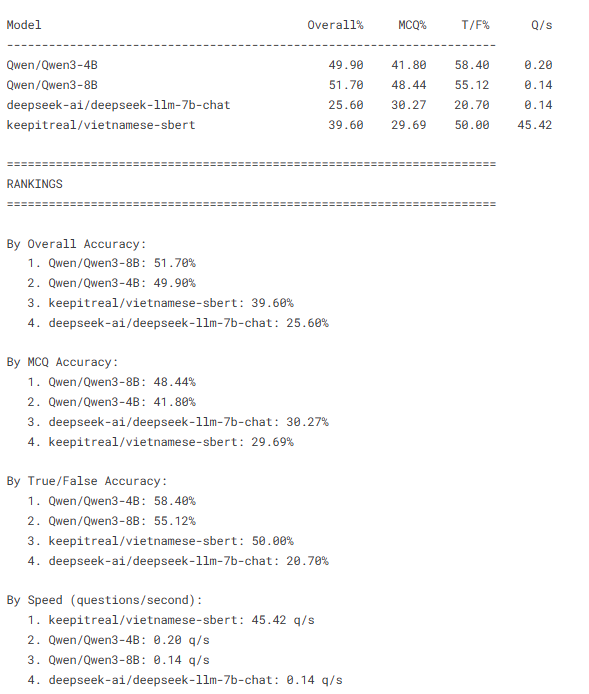
\includegraphics[width=0.75\linewidth]{Screenshot 2025-12-12 203013.png}
    \caption{Báo cáo kết quả thực hiện trả lời câu hỏi lịch sử với LLMs}
    \label{fig:placeholder}
\end{figure}

\begin{table}[H]
\centering
\caption{Xếp hạng mô hình theo tiêu chí}
\label{tab:model-ranking}
\begin{tabular}{|c|c|c|c|c|}
\hline
\textbf{Hạng} & \textbf{Tổng thể} & \textbf{MCQ} & \textbf{TF} & \textbf{Tốc độ} \\
\hline
1 & Qwen3-8B & Qwen3-8B & Qwen3-4B & Viet-SBERT \\
2 & Qwen3-4B & Qwen3-4B & Qwen3-8B & Qwen3-4B \\
3 & Viet-SBERT & DeepSeek-7B & Viet-SBERT & Qwen3-8B \\
4 & DeepSeek-7B & Viet-SBERT & DeepSeek-7B & DeepSeek-7B \\
\hline
\end{tabular}
\end{table}

Qwen3-8B đạt độ chính xác tổng thể cao nhất (51.70\%), vượt trội so với DeepSeek-7B (25.60\%) và Vietnamese-SBERT (39.60\%). Mặc dù yêu cầu thời gian xử lý lâu hơn, Qwen3-8B bù đắp bằng khả năng tuân thủ định dạng đầu ra (0\% null) và hiệu năng cân bằng trên cả hai loại câu hỏi. DeepSeek-7B có tỷ lệ null prediction cao nhất (32.4\%) và độ chính xác thấp nhất, đặc biệt với câu hỏi TF (20.70\%). Vietnamese-SBERT tuy nhanh hơn đáng kể (45.42 q/s) nhưng kém hiệu quả với MCQ (29.69\%) do phương pháp embedding không phù hợp cho câu hỏi yêu cầu suy luận.

Từ kết quả thực nghiệm, rút ra ba nhận xét chính: (1) Độ chính xác tối đa ~52\% cho thấy LLM không có tri thức bổ sung chưa đủ tin cậy cho bài toán này; (2) Qwen3-4B chỉ kém 1.8\% so với Qwen3-8B nhưng tiết kiệm 50\% tài nguyên, phù hợp cho triển khai thực tế; (3) Kết quả đặt ra yêu cầu tích hợp nguồn tri thức bên ngoài thông qua RAG hoặc GraphRAG để cải thiện độ chính xác.
\newpage
\subsection{Thực nghiệm với RAG}

Phần này trình bày chi tiết thực nghiệm sử dụng phương pháp RAG để nâng cao hiệu suất của mô hình ngôn ngữ trong bài toán trả lời câu hỏi lịch sử Việt Nam. Mục tiêu là đánh giá khả năng của hệ thống khi được bổ sung cơ chế truy xuất thông tin từ một kho tài liệu có cấu trúc (sách giáo khoa).

\paragraph{Cấu hình thực nghiệm}
Hệ thống RAG được triển khai với cấu hình cụ thể được tóm tắt trong Bảng \ref{tab:rag-config}. Cấu hình này được tối ưu để cân bằng giữa hiệu năng, độ chính xác và tài nguyên tính toán sẵn có.

\begin{table}[H]
\centering
\caption{Cấu hình hệ thống RAG}
\label{tab:rag-config}
\begin{tabular}{|l|l|}
\hline
\textbf{Thành phần} & \textbf{Cấu hình} \\
\hline
Môi trường thực thi & Kaggle Notebook, 2x NVIDIA T4 (16GB VRAM) \\
Mô hình sinh (Generator) & Qwen3-4B (bfloat16) \\
Mô hình nhúng (Embedding) & Qwen3-Embedding-0.6B \\
Vector Database & FAISS với IndexFlatIP \\
Kích thước chunk tối đa & 500 ký tự \\
Ngưỡng điểm tối thiểu & 0.35 \\
Số chunks tối đa cho context & 2 \\
Độ dài context tối đa & 1,200 ký tự \\
Top-k retrieval (câu hỏi) & 1 \\
Top-k retrieval (từ khóa) & 1 \\
\hline
\end{tabular}
\end{table}

\paragraph{Kiến trúc Hệ thống RAG:}
Hệ thống được triển khai theo kiến trúc ba tầng chức năng chính, hoạt động tuần tự để xử lý một truy vấn:

\begin{enumerate}
    \item \textbf{Indexing Layer:} Chịu trách nhiệm tiền xử lý và chuẩn bị kho tri thức.
    \begin{itemize}
        \item \textit{Text Chunking:} Nội dung sách giáo khoa được chia thành các đoạn nhỏ, tối đa 500 ký tự, với điểm cắt ưu tiên giữa các câu để đảm bảo tính nguyên vẹn về ngữ nghĩa.
        (\texttt{lesson\_id}), tiêu đề chương và mục.
        \item \textit{Embedding:} Mỗi đoạn văn được chuyển thành biểu diễn vector 1024 chiều sử dụng mô hình \texttt{Qwen3-Embedding-0.6B}.
        \item \textit{Vector Store:} Toàn bộ vector được lưu trữ và lập chỉ mục trong FAISS, sử dụng Inner Product để tìm kiếm tương đồng.
    \end{itemize}

    \item \textbf{Retrieval Layer:} Thực hiện tìm kiếm thông tin liên quan khi nhận truy vấn.
    \begin{itemize}
        \item \textit{Semantic Search:} Mã hóa câu hỏi thành vector và tìm kiếm các đoạn văn có embedding gần nhất trong không gian vector.
        \item \textit{Keyword Search:} Bổ sung kết quả bằng cách tìm kiếm trực tiếp trên các từ khóa quan trọng được trích xuất từ câu hỏi.
        \item \textit{Score Filtering:} Chỉ giữ lại các đoạn văn có điểm tương đồng vượt ngưỡng 0.35.
        \item \textit{Context Aggregation:} Các đoạn văn được chọn sẽ được ghép nối, với tổng độ dài không vượt quá 1,200 ký tự, để tạo thành ngữ cảnh đầu vào cho bước tiếp theo.
    \end{itemize}

    \item \textbf{Generation Layer:} Tổng hợp thông tin và tạo ra câu trả lời cuối cùng.
    \begin{itemize}
        \item \textit{Augmented Prompt Construction:} Ngữ cảnh được truy xuất ($C$) được kết hợp với câu hỏi gốc ($question$) theo một khuôn mẫu được thiết kế sẵn.
        \item \textit{LLM Inference:} Prompt hoàn chỉnh được đưa vào mô hình sinh \texttt{Qwen3-4B} để tạo phản hồi văn bản.
        \item \textit{Post-processing:} Đáp án dạng chữ cái (A/B/C/D) hoặc "Đúng"/"Sai" được trích xuất tự động từ đầu ra văn bản của mô hình.
    \end{itemize}
\end{enumerate}

\paragraph{Prompt Enginerring cho RAG:} Để hướng dẫn LLM sử dụng hiệu quả ngữ cảnh được truy xuất, các mẫu prompt chuyên biệt được thiết kế cho từng loại câu hỏi.

\begin{lstlisting}[language=Python, caption={Prompt template cho câu hỏi trắc nghiệm với RAG}]
PROMPT = """Dua vao kien thuc duoc dua. Kiem tra thong tin 
sau va tra loi cau hoi. Neu thieu thong tin hoac khong 
ro rang tra loi bang du lieu hien co.
THONG TIN:
{context}
CAU HOI: {question}
CAC DAP AN:
{options}
Dua vao thong tin tren, chon dap an phu hop nhat.
DAP AN:"""
\end{lstlisting}
\textbf{Template cho câu hỏi True/False với context:}
\begin{lstlisting}[language=Python, caption={Prompt template cho câu hỏi đúng/sai với RAG}]
PROMPT = """Ban la mot chuyen gia ve lich su Viet Nam va 
the gioi. Hay doc ky phat bieu sau va xac dinh xem no 
DUNG hay SAI.
Phat bieu: {question}
Hay phan tich ngan gon va dua ra ket luan. 
Tra loi bang "Dung" neu phat bieu dung, 
hoac "Sai" neu phat bieu sai.
Ket luan:"""
\end{lstlisting}
\paragraph{Thống kê Kho tri thức và Hiệu năng}
Kho tri thức được xây dựng từ sách giáo khoa và các chỉ số hiệu năng liên quan được trình bày trong Bảng \ref{tab:vector-store-stats}.

\begin{table}[H]
\centering
\caption{Thống kê Kho dữ liệu Vector và Hiệu năng Truy xuất}
\label{tab:vector-store-stats}
\begin{tabular}{|>{\raggedright}p{7cm}|c|}
\hline
\textbf{Chỉ số} & \textbf{Giá trị} \\ \hline
Tổng số đoạn văn bản (chunks) trong kho dữ liệu & 340 \\ \hline
Chiều của vector embedding & 1024 \\ \hline
Thời gian mã hóa toàn bộ kho dữ liệu (batch size = 64) & $\sim$30 giây \\ \hline
Thời gian truy xuất trung bình cho một câu hỏi & < 50 mili giây \\ \hline
\end{tabular}
\end{table}

\paragraph{Kết quả:}
Hệ thống được đánh giá trên cùng bộ dữ liệu 1,000 câu hỏi được tạo trước đó. Kết quả chi tiết được trình bày trong Bảng \ref{tab:rag-results-detail}.

\begin{table}[H]
\centering
\caption{Kết quả đánh giá chi tiết hệ thống RAG + Qwen3-4B}
\label{tab:rag-results-detail}
\begin{tabular}{|l|c|c|c|c|}
\hline
\textbf{Loại câu hỏi} & \textbf{Số câu đúng} & \textbf{Tổng số câu} & \textbf{Độ chính xác (\%)} & \textbf{Thời gian xử lý TB (giây)} \\ \hline
Trắc nghiệm (MCQ) & 322 & 512 & 62.9 & 2.6 \\ \hline
Đúng/Sai (True/False) & 258 & 488 & 52.9 & 1.7 \\ \hline
\textbf{Tổng hợp} & \textbf{580} & \textbf{1,000} & \textbf{58.0} & \textbf{2.2} \\ \hline
\end{tabular}
\end{table}

\noindent\textbf{Thống kê hiệu suất tổng thể:}
\begin{itemize}
    \item Tổng thời gian chạy đánh giá: 38 phút 25 giây.
    \item Tốc độ xử lý trung bình: 26 câu hỏi/phút.
    \item Tỷ lệ có thể trích xuất được đáp án: 100\%.
\end{itemize}

\paragraph{So sánh với Phương pháp Sử dụng LLMs}
Để đánh giá hiệu quả của cơ chế RAG, kết quả được so sánh trực tiếp với phương pháp zero-shot sử dụng chính mô hình \texttt{Qwen3-4B} mà không có truy xuất ngữ cảnh. Kết quả so sánh được trình bày trong Bảng \ref{tab:rag-vs-zeroshot}.

\begin{table}[H]
\centering
\caption{So sánh Độ chính xác giữa Phương pháp RAG và Zero-shot (sử dụng Qwen3-4B)}
\label{tab:rag-vs-zeroshot}
\begin{tabular}{|l|c|c|c|}
\hline
\textbf{Phương pháp} & \textbf{MCQ (\%)} & \textbf{True/False (\%)} & \textbf{Tổng thể (\%)} \\ \hline
Zero-shot (Qwen3-4B) & 41.8 & 58.4 & 49.9 \\ \hline
RAG + Qwen3-4B & 62.9 & 52.9 & 58.0 \\ \hline
\textbf{Mức cải thiện} & \textbf{+21.1} & \textbf{-5.9} & \textbf{+8.1} \\ \hline
\end{tabular}
\end{table}

\paragraph{Phân tích và Thảo luận}
Kết quả thực nghiệm cho thấy một số điểm đáng chú ý:
\begin{itemize}
    \item \textbf{Cải thiện vượt trội với Câu hỏi MCQ:} Độ chính xác tăng 21.1\%, chứng tỏ RAG đặc biệt hiệu quả khi câu hỏi yêu cầu truy xuất thông tin sự kiện, ngày tháng, hoặc dữ kiện cụ thể từ kho tài liệu.
    \item \textbf{Cải thiện khiêm tốn với Câu hỏi Đúng/Sai:} Mức giảm 5.9\% cho thấy các câu hỏi dạng này thường yêu cầu suy luận hoặc đánh giá logic phức tạp hơn nhưng đồng thời có thêm phần dữ kiện trước đó khiến gặp nhiễu khi xử lý câu hỏi dạng này. 
    \item \textbf{Ưu điểm của RAG:} Phương pháp này giúp giảm thiểu đáng kể hiện tượng hallucination của LLM bằng cách ràng buộc câu trả lời vào ngữ cảnh có kiểm chứng. Hệ thống cũng có tính linh hoạt cao, dễ dàng cập nhật tri thức mới mà không cần huấn luyện lại mô hình, đồng thời cung cấp khả năng truy vết nguồn gốc thông tin.
    \item \textbf{Hạn chế và Hướng phát triển:} Hiệu năng của hệ thống phụ thuộc nhiều vào chất lượng bước truy xuất. Các câu hỏi đòi hỏi kết nối thông tin từ nhiều nguồn. Ngoài ra, sự khác biệt trong cách diễn đạt giữa câu hỏi và văn bản nguồn có thể tạo ra semantic gap. Các hạn chế này chính là động lực để nghiên cứu và phát triển tiếp phương pháp GraphRAG, được trình bày trong phần tiếp theo, với kỳ vọng khắc phục thông qua việc sử dụng cấu trúc đồ thị tri thức.
\end{itemize}